\section{Animal identification by time-frequency analysis}
\subsection{Listen and identify:}
The animal call sounds very synthetic. We therefore examine the spectrum to see if it 
will reveal some useful information. After reducing the window size it turns out that
the animal call can only be produced by either the illusive \emph{Coffee Arabica Bibentum igenarius}
or the lyrebird which is capable of mimicing almost any sound it encounters, including chainsaws,
camera shutters, car alarms and more.\footnote{For proof see David Attenborough on the lyrebird \url{https://www.youtube.com/watch?v=VjE0Kdfos4Y}}
Figure~\ref{fig:zebra} shows the animal hidden in the spectrum.
\begin{figure}
	\center
	\includegraphics{./picture/zebra.eps}
	\caption{The hidden zebra in grayscale for printer friendliness.}
	\label{fig:zebra}
\end{figure}
